\documentclass[journal]{IEEEtran}
\usepackage[margin=1in]{geometry}
\pdfinfoomitdate=1
\pdftrailerid{}
\pdfsuppressptexinfo=-1
\usepackage{amsmath,amssymb,amsthm,bm}
\usepackage{booktabs}
\usepackage{graphicx}
\usepackage{cite}
\usepackage{url}
\usepackage{algorithmic}
\usepackage[hidelinks]{hyperref}
\newtheorem{assumption}{Assumption}
\newtheorem{theorem}{Theorem}
\newtheorem{proposition}{Proposition}
\newtheorem{lemma}{Lemma}
\newtheorem{corollary}{Corollary}
\newcommand{\E}{\mathbb{E}}
\newcommand{\Pp}{\mathbb{P}}
\newcommand{\R}{\mathbb{R}}
\newcommand{\A}{\mathcal{A}}
\newcommand{\F}{\mathcal{F}}
\newcommand{\KL}{\operatorname{KL}}
\newcommand{\TV}{\operatorname{TV}}
\newcommand{\tr}{\operatorname{tr}}
\title{Learning-Aware Lyapunov Resource Control for Correlated Multi-Agent Markov Learning}
\author{Jialin~Zhuang,~\IEEEmembership{Member,~IEEE,}
and~Vincent~K.~N.~Lau,~\IEEEmembership{Fellow,~IEEE}%
\thanks{J.~Zhuang and V.~Lau are with the Department of Electronic and Computer Engineering, The Hong Kong University of Science and Technology, Clear Water Bay, Hong Kong SAR, China (e-mail: \mbox{jzhuangag@connect.ust.hk}; \mbox{eeknlau@ece.ust.hk}).
This work was supported by the Research Grants Council (RGC), Hong Kong, under the Areas of Excellence Scheme Grant AoE/E-101/23-N and AoE/E-601/22-R.
(\em{Corresponding author: Vincent K. N. LAU}.)}
}
\begin{document}
\maketitle
\begin{abstract}
Parallel policy evaluation depends on cross-agent correlation, temporal persistence, communication, and update staleness.
We formulate allocation as finite-budget learning-value control: a server selects participation, sample spacing, and step size before an update.
A discrete Lyapunov certificate converts these decisions into a terminal-risk objective for affine delayed temporal-difference learning.
Its terms retain cross-agent second moments, finite-mixing bias, and the delay profile, so the certificate both proves convergence and designs the resource action.
When dependence is unknown, a learning-aware gate purchases a fully charged likelihood probe only when its certified downstream risk reduction exceeds message, transition, delay, and decision-error costs.
We establish a stopped adaptive change-of-measure lower bound, a finite-horizon performance and safety theorem, and a necessary--sufficient budget-threshold sandwich on a separated Markov class.
Controlled studies recover correlation-limited speedup, calibrate the finite-time bounds, and reduce two finite-budget risks by 35.2 and 9.8 percent relative to information-only probing.
On 64 held-out seeds, joint control reduces parameter-error and discounted-return-estimation curve integrals by 9.9 and 11.3 percent against a development-selected fixed baseline.
Held-out multi-agent proximal policy optimization studies on particle coordination and locomotion select dependence-matched participation in all 32 controller runs.
Under identical charged budgets, the controller improves mean normalized team-return curve integrals by 2.32 percent on particles and paired equal-mixture integrals by 8.34 percent on locomotion over the strongest single fixed-participation comparators.
\end{abstract}
\begin{IEEEkeywords}
Multi-agent learning, Markov data, temporal-difference learning, adaptive sensing, Lyapunov methods.
\end{IEEEkeywords}

\section{Introduction}
Policy evaluation estimates the discounted return of a fixed policy, supplying the critics and advantages used by actor--critic systems.
We study parallel actors executing a common target policy on Markov environment copies and sending temporal-difference observations to a value-learning server.
The server chooses participation $q$, physical sample spacing $b$, and step size $\eta$ under finite message and environment-clock budgets.

Parallel samples need not provide parallel information: actors can share simulator randomness or exogenous disturbances while preserving their marginal transition laws.
At correlation $\rho>0$, equicorrelated Gaussian observations provide effective participation $q/[1+(q-1)\rho]\le1/\rho$, while messages grow with $q$.
Larger spacing suppresses Markov bias but consumes transitions; larger steps accelerate contraction but raise noise and stale-update risk.
The design must price these effects against the affordable learning horizon and dependence-identification cost.

Temporal-difference and stochastic-approximation foundations~\cite{sutton1988td,tsitsiklis1997td,robbins1951stochastic,polyak1992averaging} lead to finite-time Markov analyses~\cite{bhandari2018finite,srikant2019finite,mou2022optimal}, concentration tools~\cite{paulin2015concentration}, and Lyapunov-based adaptive rates~\cite{gupta2019adaptive}.
Our design also controls the spatial participation and sampling clock creating the observation stream.

Distributed/federated learning studies consensus, parallelism, coverage, and sample--communication tradeoffs~\cite{doan2019distributed,zhang2018decentralized,khodadadian2022federated,woo2023heterogeneity,salgia2024tradeoff,lan2023communication}.
Clustered clients, adaptive batches, and antithetic sampling regulate variance~\cite{fraboni2021clustered,de2017adaptive,ren2019antithetic}; feedback controls participation~\cite{cummins2025feedback}, while convergence-bound-driven Lyapunov control selects clients and powers~\cite{perazzone2025lyapunov}.
Our learning-risk score instead couples cross-agent covariance and Markov spacing to stable step adaptation and the action-dependent number of affordable future updates.

Asynchronous optimization prices stale computation~\cite{agarwal2011distributed,lian2015asynchronous,arjevani2020delayed}; Markov delay-adaptive approximation~\cite{adibi2024delayed,dalfabbro2024dasa} and stochastic delay differential equations (SDDEs) extend convergence and worker-activation design~\cite{yu2025sdde}.
We additionally price the message, transition, and noise cost of correlated trajectories.

Sequential design and identification supply change-of-measure/allocation tools~\cite{chernoff1959sequential,nitinawarat2015controlled,kaufmann2016complexity,garivier2016optimal,moulos2019markovian,saad2023covariance,vannella2023multiagent}, with conservative bandits constraining baseline-relative reward~\cite{wu2016conservative}.
Here identification is valued through the remaining learner's risk.
We jointly control these quantities through an action-dependent Lyapunov certificate composed over the affordable updates.
The resulting terminal-risk score supports scalar step searches within each discrete $(q,b)$ pair.
For unknown dependence, a likelihood probe is admitted when its certified downstream improvement exceeds message, transition, delay, and decision-error costs while respecting a low-instance risk allowance.

The main contributions are as follows.
\begin{itemize}
\begin{samepage}
\item \textbf{Finite-Budget Learning-Value Formulation:} We jointly control spatial participation, physical Markov spacing, and step size under dual budgets, with an exact correlation-limited Gaussian speedup ceiling.
\par
\end{samepage}
\item \textbf{Lyapunov-Certified Resource Control:} An affine delayed Markov certificate supplies the joint score, uniform-history critic tracking, and conservative-certificate risk and selection-sensitivity guarantees.
\item \textbf{Information-to-Learning Phase Characterization:} A stopped adaptive information identity and controlled-belief occupation program lower-bound identification cost; a learning-value gate yields finite-budget risk guarantees and a threshold sandwich on a separated Gaussian class.
\item \textbf{Charged Learning Evidence:} Controlled studies reduce risk by 35.2 and 9.8 percent relative to information-only probing and held-out parameter/return-estimation area under the curve (AUC) by 9.9/11.3 percent versus a development-selected fixed baseline.
Held-out multi-agent proximal policy optimization (MAPPO) studies improve particle mean normalized team-return AUC by 2.32 percent and locomotion paired equal-mixture AUC by 8.34 percent versus the strongest single fixed actions, with all 32 controller runs selecting dependence-matched participation.
\end{itemize}

The remainder of the paper develops the argument as follows.
Sections~II--IV define the model and derive its resource geometry and Lyapunov controller; Sections~V--VI establish adaptation and implementation; Sections~VII--VIII present simulations and conclusions.

\section{Model and Finite-Budget Objective}
\subsection{Fixed-policy evaluation with multiple actors}
Let $({\cal S},{\cal U},P,r,\gamma)$ be a discounted Markov decision process and let $\pi_{\rm tar}(u\mid s)$ be a fixed target policy.
Under $\pi_{\rm tar}$, the state--action process is a Markov reward process with transition kernel $P_{\pi}$ and stationary distribution $\pi$.
For a feature vector $\phi(s)\in\R^d$, the linear value approximation is $V_w(s)=\phi(s)^\top w$.
Its projected Bellman fixed point $w^\star$ solves
\begin{equation}
A w^\star=c,
\quad
A=\E_\pi[\phi_t(\phi_t-\gamma\phi_{t+1})^\top],
\quad
c=\E_\pi[r_t\phi_t].
\label{eq:projected-fixed-point}
\end{equation}

Let $S_k$ be the start of retained transition $k$ and $X_{i,k}=(s_{i,S_k},r_{i,S_k},s_{i,S_k+1})$.
The server chooses $q_k\in\{1,\ldots,Q\}$ actors and start-to-start spacing $b_k\in\mathbb N$.
For temporal-difference data, $P_q$ is a Markov augmentation containing the joint transition tuples, not the raw state kernel; retained starts are separated by $b_k$ kernel steps.
Its invariant law $\pi_q$ satisfies the total-variation (TV) bound
\begin{equation}
\sup_z\left\|P_q^b(z,\cdot)-\pi_q\right\|_{\rm TV}\le C_qr_q^b,
\quad 0<r_q<1.
\label{eq:mixing}
\end{equation}
Every actor has the target-policy marginal law; cross-agent dependence enters the aggregate stationary moments.

For the identification layer, a Gaussian common-factor subclass makes the dependence parameter explicit.
Under instance $j\in\{0,1\}$,
\begin{align}
C_{S_k}&=\lambda^{b_k}C_{S_{k-1}}+\sqrt{1-\lambda^{2b_k}}\,\xi_{j,k},\nonumber\\
X_{i,k}&=C_{S_k}+\epsilon_{i,k},
\label{eq:common-factor}
\end{align}
where $\xi_{j,k}\sim\mathcal{N}(0,\theta_j)$, $\epsilon_{i,k}\sim\mathcal{N}(0,1)$, and all private innovations are independent.
The common process is initialized with $C_{S_0}\sim\mathcal N(0,\theta_j)$; fixed-clock probes are stationary, whereas adaptive sampling need not preserve that marginal.
The corresponding same-time correlation is $\rho_j=\theta_j/(1+\theta_j)$.
Within each instance, every actor has the same marginal law; changing $\theta_j$ changes both marginal variance and cross-agent correlation.
It is used to prove the information boundary; the convergence theorem below applies to bounded affine temporal-difference observations satisfying Assumption~\ref{ass:catalogue}.

\subsection{Affine delayed temporal-difference recursion}
Let $w^\star\in\R^d$ be the projected temporal-difference fixed point and $e_k=w_k-w^\star$.
For action $a=(q,b,\eta)$ and delays $0\le\tau_i\le D$, the retained recursion is
\begin{equation}
e_{k+1}=e_k-\frac{\eta}{q}\sum_{i=1}^{q}\left(H_{i,k}e_{k-\tau_i}-\xi_{i,k}\right).
\label{eq:affine-td}
\end{equation}
The rank-one matrix $H_{i,k}$ is the sample temporal-difference Jacobian and $\xi_{i,k}$ is the affine innovation at $w^\star$.
For temporal-difference (TD) learning with zero trace, TD(0), these quantities are
\begin{equation}
H_{i,k}=\phi_{i,k}(\phi_{i,k}-\gamma\phi'_{i,k})^\top,
\quad
\xi_{i,k}=\phi_{i,k}\delta_i(w^\star),
\label{eq:td-components}
\end{equation}
where $\delta_i(w)=r_{i,k}+\gamma\phi_{i,k}'{}^\top w-\phi_{i,k}^\top w$.
The first tuple must satisfy the same conditional mixing bound, or be initialized independently from stationarity.

\begin{assumption}[Certified action domain]
The public sets ${\cal Q}\subseteq\{1,\ldots,Q\}$ and ${\cal B}\subset\mathbb N$ are finite, while the step interval $[\eta_{\min},\eta_{\max}]$ is compact.
For each $a=(q,b,\eta)$ in their product: (a) $\|H_{i,k}\|\le L$ and $\|\xi_{i,k}\|\le G$ almost surely; (b) $\E_{\pi_q}\xi_{i,k}=0$, and the common mean $A=\E_{\pi_q}H_{i,k}$ has symmetric part at least $\mu I$; (c) the delay profile is deterministic, satisfies $0\le\tau_i\le D$, and is known when scoring; and (d) predictable upper bounds cover the stationary aggregate moments and the mixing law uniformly conditional on pre-observation history.
Initialize $w_s=w_0$ for all $s\le0$; increments before the first update are zero.
\label{ass:catalogue}
\end{assumption}

Write $\A={\cal Q}\times{\cal B}\times[\eta_{\min},\eta_{\max}]$; integer actor counts and clocks are enumerated, with a continuous scalar step search.

\subsection{Dual budgets and terminal risk}
Each scheduled block pays $h+q$ message units and $b$ parallel-clock units, including unused padding within the block.
Let $u\ge0$ count terminal scheduled updates excluded from the reported learner and let $\ell\ge0$ be a separately declared physical startup/drain charge.
Neither quantity is the recursion's state-lag bound $D$ unless the protocol explicitly equates them.
A feasible trajectory therefore satisfies
\begin{equation}
\sum_k(h+q_k)\le B_{\rm msg},
\quad
\sum_k b_k+\ell\mathbf{1}\{K>0\}\le B_{\rm env}.
\label{eq:budgets}
\end{equation}
For a stationary action, all scheduled blocks are paid, and the usable horizon is
\begin{equation}
N_a(B)=\left[\min\left\{\left\lfloor\frac{B_{\rm msg}}{h+q}\right\rfloor,
\left\lfloor\frac{B_{\rm env}-\ell}{b}\right\rfloor\right\}-u\right]_+.
\label{eq:usable-horizon}
\end{equation}
The controller minimizes a finite-time certificate $\overline R_j(a;B,D)$ satisfying $\E_j\|e_{N_a}\|^2\le\overline R_j(a;B,D)$.
This parameter mean-square risk controls the value-estimation risk of $J_\nu(w)=\E_{s\sim\nu}V_w(s)$, as quantified by Corollary~\ref{cor:return}.

The Gaussian running-mean learner used in the mechanism study starts from a unit pseudo-observation.
For $r=\lambda^b$, its exact risk is
\begin{align}
R_j^{\rm mean}(a,N)&=\frac{1+N/q}{(N+1)^2}\nonumber\\
&\quad+\frac{\theta_j\left[N+2\sum_{s=1}^{N-1}(N-s)r^s\right]}{(N+1)^2}.
\label{eq:mean-risk}
\end{align}
Eq.~\eqref{eq:mean-risk} exposes opposing effects: larger $q$ reduces private noise but can reduce $N$, while spacing controls $r$ at a transition cost.

\section{Correlation and Resource Geometry}
\subsection{A sharp spatial speedup ceiling}
The statistical role of participation is exact in a Gaussian location subclass.
Let $Y_{i,t}=\vartheta+C_t+\epsilon_{i,t}$ with common variance $\sigma_c^2$, private variance $\sigma_e^2$, and independent rounds.
For a fixed participation $q$, the minimax squared-error risk after $T$ rounds is
\begin{equation}
R_q(T)=\frac{1}{T}\left(\sigma_c^2+\frac{\sigma_e^2}{q}\right).
\label{eq:location-risk}
\end{equation}
Writing $\rho=\sigma_c^2/(\sigma_c^2+\sigma_e^2)$ gives the speedup relative to one actor,
\begin{equation}
S(q,\rho)=\frac{R_1(T)}{R_q(T)}
=\frac{q}{1+(q-1)\rho}
\le\min\{q,\rho^{-1}\}.
\label{eq:speedup}
\end{equation}
Thus information saturates at positive correlation while messages grow with $q$.

\begin{proposition}[Participation phase under a message budget]
Suppose the environment budget does not bind, $h>0$, $0<\rho<1$, and a message budget $B_{\rm msg}$ is used with fixed $q$.
Ignoring integer rounding, the minimax risk is proportional to
\begin{equation}
F(q;\rho,h)=(h+q)\left(\rho+\frac{1-\rho}{q}\right).
\label{eq:participation-phase-objective}
\end{equation}
Its continuous minimizer is
\begin{equation}
q_{\rm cont}^\star=\sqrt{\frac{h(1-\rho)}{\rho}},
\label{eq:participation-phase}
\end{equation}
clipped to $[1,Q]$, and an integer optimum is one of its two neighboring feasible participation levels.
\label{prop:q-phase}
\end{proposition}

Differentiating $F$ gives $\partial_qF=\rho-h(1-\rho)/q^2$, proving Proposition~\ref{prop:q-phase}.
Fixed overhead favors larger batches; common randomness favors smaller participation.

\subsection{Temporal spacing and the usable horizon}
For the common-factor process in Eq.~\eqref{eq:common-factor}, retaining every $b$th observation changes persistence from $\lambda$ to $r=\lambda^b$.
The integrated correlation term in Eq.~\eqref{eq:mean-risk} admits the closed form
\begin{equation}
\sum_{s=1}^{N-1}(N-s)r^s
=\frac{r\{(N-1)-Nr+r^N\}}{(1-r)^2}.
\label{eq:geometric-correlation-sum}
\end{equation}
For nonnegative persistence, increasing $b$ suppresses the positive correlation term, but Eq.~\eqref{eq:usable-horizon} decreases approximately as $1/b$ when the environment clock binds.
Consequently, aggressive thinning can make retained observations nearly independent and still increase terminal error.

The next section jointly prices noise and contraction over this affordable horizon.

\section{Lyapunov-Certified Joint Resource Control}
\subsection{Action-dependent one-block drift}
The base Lyapunov function is the squared parameter error $V(e)=\|e\|^2$.
Delay prevents its one-step drift from closing in $e_k$ alone because the update also contains $e_{k-\tau_i}$.
We therefore analyze the observable-independent sliding envelope
\begin{equation}
R_k=\max_{k-2D\le s\le k}\E V(e_s),
\label{eq:sliding-envelope}
\end{equation}
which is a Lyapunov--Razumikhin construction for the lifted history $(e_k,e_{k-1},\ldots,e_{k-2D})$.

Define the aggregate stationary moments
\begin{equation}
K_q=\lambda_{\max}\!\left(\E_{\pi_q}[\bar H_k^\top\bar H_k]\right),
\quad
\Omega_q=\E_{\pi_q}\|\bar\xi_k\|^2,
\end{equation}
where $\bar H_k=q^{-1}\sum_iH_{i,k}$ and $\bar\xi_k=q^{-1}\sum_i\xi_{i,k}$.
Let $\delta=C_qr_q^b$ and $\mu_\delta=\mu-2L\delta$.
For the delay root-mean-square $\tau_{\rm rms}=(q^{-1}\sum_i\tau_i^2)^{1/2}$, define
\begin{align}
a_\delta(\eta)&=1-\eta\mu_\delta+\eta^2(2K_q+4L^2\delta),\nonumber\\
\beta_\delta(\eta)&=\frac{4\eta G^2\delta^2}{\mu_\delta}+\eta^2(2\Omega_q+4G^2\delta),\nonumber\\
h_\tau(\eta)&=2\eta^4L^4\tau_{\rm rms}^2,
\quad
g_\tau(\eta)=2\eta^4L^2G^2\tau_{\rm rms}^2.
\label{eq:affine-terms}
\end{align}
For positive delay, set $\lambda_\star=\sqrt{h_\tau/a_\delta}$ and
\begin{align}
c_{\rm aff}&=(1+\lambda_\star)a_\delta+(1+\lambda_\star^{-1})h_\tau,\nonumber\\
d_{\rm aff}&=(1+\lambda_\star)\beta_\delta+(1+\lambda_\star^{-1})g_\tau.
\label{eq:affine-cd}
\end{align}
The zero-delay definitions are the continuous limits $c_{\rm aff}=a_\delta$ and $d_{\rm aff}=\beta_\delta$.
The coefficients price mean drift, multiplicative/additive sampling noise, finite mixing, and fourth-order stale-state substitution.

\begin{theorem}[Affine delayed Markov Lyapunov bound]
Suppose Assumption~\ref{ass:catalogue} holds, $\mu_\delta>0$, $a_\delta(\eta)>0$, and $c_{\rm aff}(a)<1$.
Let $m=2D+1$ and $R_k=\max_{k-2D\le s\le k}\E\|e_s\|^2$.
Then, for every integer $n\ge0$,
\begin{equation}
R_{nm}\le c_{\rm aff}(a)^nR_0+\frac{d_{\rm aff}(a)}{1-c_{\rm aff}(a)}.
\label{eq:affine-bound}
\end{equation}
\label{thm:affine}
\end{theorem}
Appendix~\ref{app:affine} proves the bound: correlation enters $(K_q,\Omega_q)$, persistence enters $\delta$, and delay changes contraction and forcing.

\begin{corollary}[Finite-horizon return certificate]
Under Theorem~\ref{thm:affine}, let $n=\lfloor N_a(B)/(2D+1)\rfloor$ and let $\psi_\nu=\E_{s\sim\nu}\phi(s)$.
Then
\begin{equation}
\E\left|J_\nu(w_{N_a})-J_\nu(w^\star)\right|^2
\le \|\psi_\nu\|^2
\left[c_{\rm aff}^{n}R_0+\frac{d_{\rm aff}}{1-c_{\rm aff}}\right].
\label{eq:return-certificate}
\end{equation}
\label{cor:return}
\end{corollary}

Appendix~\ref{app:return} handles incomplete terminal blocks and connects parameter risk to fixed-policy value-estimation error.

The same certificate also tracks a critic target moved by a policy learner.
Let $w_r^\star$ be the projected fixed point during epoch $r$, lasting one replacement block $m=2D+1$, and let $Z_r=\max_{rm-2D\le s\le rm}\E\|w_s-w_r^\star\|^2$.

\begin{theorem}[Moving-policy critic tracking]
Suppose every epoch satisfies Assumption~\ref{ass:catalogue}, possibly with a different certified action $a_r$, and its coefficients obey $c_{\rm aff}(a_r)\le c<1$ and $d_{\rm aff}(a_r)\le d$.
Require the fixed-target one-step inequality $\E\|w_{k+1}-w_r^\star\|^2\le c\max_{k-2D\le s\le k}\E\|w_s-w_r^\star\|^2+d$ throughout epoch $r$, including its mixed-history boundary.
This requirement holds for a consistently initialized epoch with no carried old-target updates; without that protocol it is an additional uniform-history condition.
If the policy-induced target moves only between epochs and
$\|w_{r+1}^\star-w_r^\star\|\le v$, then for every $\chi>0$ satisfying $\bar c=(1+\chi)c<1$,
\begin{align}
Z_n&\le \bar c^n Z_0+
\frac{(1+\chi)d+(1+\chi^{-1})v^2}{1-\bar c},\label{eq:tracking-bound}\\
\E|\widehat A_w-A^\star|^2
&\le (1+\gamma)^2\Phi^2 Z_n,\quad \|\phi(s)\|\le\Phi.
\label{eq:advantage-transfer}
\end{align}
\label{thm:tracking}
\end{theorem}

The bound exposes a moving-target phase: policy improvement increases $v$, while the resource action determines $(c,d)$.
Appendix~\ref{app:tracking} proves the positive-part recursion.
Under the uniform-history condition, recomputing the joint score at actor-epoch boundaries controls the certified critic lag.

\subsection{Joint action selection}
For $n_a=\lfloor N_a(B)/m\rfloor$, the certificate score is
\begin{equation}
\mathcal{U}_j(a;B,D)=R_\star(a)+c_{\rm aff}(a)^{n_a}\left(R_0-R_\star(a)\right)_+,
\label{eq:certificate-score}
\end{equation}
where $R_\star(a)=d_{\rm aff}(a)/(1-c_{\rm aff}(a))$.
The certified oracle for a known dependence instance is
\begin{equation}
a_j^\star(B,D)\in\arg\min_{a\in\A}\mathcal{U}_j(a;B,D).
\label{eq:catalogue-oracle}
\end{equation}
For every pair $(q,b)$, define the certified scalar domain
\begin{multline}
{\cal E}_{q,b}=\{\eta\in[\eta_{\min},\eta_{\max}]:
\mu_\delta\ge\mu_0>0,\\
a_\delta(\eta)\ge a_0>0,\ c_{\rm aff}(q,b,\eta)\le1-\kappa\},
\label{eq:certified-step-domain}
\end{multline}
The controller solves
\begin{align}
\eta_{q,b}^\star\in\arg\min_{\eta\in{\cal E}_{q,b}}
&\mathcal U_j(q,b,\eta;B,D),\nonumber\\
(q^\star,b^\star)&\in\arg\min_{q,b}
\mathcal U_j(q,b,\eta_{q,b}^\star;B,D).
\label{eq:mixed-controller}
\end{align}
Here $\eta_{\min}>0$, and $\mu_0,a_0,\kappa$ are declared positive certification margins.
Pairs with empty scalar domains are omitted; at least one nonempty domain is required, otherwise the controller returns a declared feasible fallback or performs no update.
Scalar minima are ideal global solutions; a numerical bounded search yields candidates unless its global accuracy is certified.

\begin{proposition}[Existence and computation]
If $K_q$, $\Omega_q$, and the mixing certificates are finite and the declared certified domain is nonempty, then $\mathcal U_j$ is continuous on its compact scalar domains and attains a minimum.
With $N_q=|{\cal Q}|$, $N_b=|{\cal B}|$, and $L_\eta$ scalar evaluations per search, the certificate cost is $O(N_qN_bL_\eta)$ arithmetic after the moment table is cached.
For rank-one temporal-difference samples, update aggregation costs $O(qd)$ arithmetic and $O(d)$ working memory per retained block; exact spectral moment calibration is a separate cost.
\label{prop:computation}
\end{proposition}

Appendix~\ref{app:existence} proves compactness and separates aggregation from spectral calibration.

\subsection{Why minimizing one-step drift is insufficient}
A purely myopic drift rule would minimize $c_{\rm aff}(a)R_k+d_{\rm aff}(a)$.
Such a rule can prefer a large $q$ or $b$ even when its resource cost leaves too few future contractions.
Eq.~\eqref{eq:certificate-score} instead composes the drift over the action-dependent horizon in Eq.~\eqref{eq:usable-horizon}.

\section{Learning-Aware Dependence Adaptation}
\subsection{Adaptive information lower bound}
When $\theta_j$ is unknown, the controller may choose a predictable sequence $A_k=(q_k,b_k,\eta_k)$ and stop at a budget-bounded stopping time $\tau$.
Rotating $X_k$ into its normalized agent mean $Y_k=q_k^{-1/2}\bm{1}^\top X_k$ and orthogonal contrasts shows that only $Y_k$ contributes to the likelihood ratio.
Under hypothesis $j$, a scalar Kalman filter gives the predictive mean $m^-_{j,k}$ and variance $P^-_{j,k}$, with innovation variance $V_{j,k}=1+q_kP^-_{j,k}$.

Let $Z_k=(m^-_{0,k},P^-_{0,k},m^-_{1,k},P^-_{1,k})$.
The conditional directional information is
\begin{equation}
\begin{aligned}
\mathcal{I}_{01}(Z_k,A_k)=\frac12\bigg[&\log\frac{V_{1,k}}{V_{0,k}}-1\\
&+\frac{V_{0,k}+q_k(m^-_{0,k}-m^-_{1,k})^2}{V_{1,k}}\bigg].
\end{aligned}
\label{eq:conditional-kl}
\end{equation}

The dependence of information on the resource action is already visible under a fixed probe.
Let $T_n(r)$ be the $n\times n$ Toeplitz matrix with entries $[T_n(r)]_{uv}=r^{|u-v|}$, and let $\zeta_1,\ldots,\zeta_n$ be its eigenvalues.

\begin{proposition}[Exact fixed-probe information]
For a fixed probe $(q,b,n)$ with $r=\lambda^b$, the directional Kullback--Leibler (KL) divergence is
\begin{equation}
\KL(P_0^{q,b,n}\|P_1^{q,b,n})
=\frac12\sum_{\ell=1}^n
\left[x_\ell-1-\log x_\ell\right],
\label{eq:fixed-probe-kl}
\end{equation}
where $x_\ell=(1+q\theta_0\zeta_\ell)/(1+q\theta_1\zeta_\ell)$.
The Bhattacharyya exponent used by the upper rule is
\begin{equation}
I_B(q,b,n)=\frac12\sum_{\ell=1}^n
\log\frac{1+q(\theta_0+\theta_1)\zeta_\ell/2}
{\sqrt{(1+q\theta_0\zeta_\ell)(1+q\theta_1\zeta_\ell)}}.
\label{eq:bhattacharyya}
\end{equation}
\label{prop:fixed-information}
\end{proposition}

They follow by diagonalizing the common-mode covariance $I+q\theta_jT_n(r)$; the orthogonal spatial contrasts have identical laws under both hypotheses.
Participation scales common-mode eigenvalues rather than creating independent temporal records.

\begin{theorem}[Stopped adaptive information identity]
If the action kernel is predictable and common to both hypotheses and $\tau$ is bounded by Eq.~\eqref{eq:budgets}, then
\begin{equation}
\KL(P_0^\pi|\F_\tau\,\|\,P_1^\pi|\F_\tau)=\E_0^\pi\sum_{k=1}^{\tau}\mathcal{I}_{01}(Z_k,A_k).
\label{eq:adaptive-kl}
\end{equation}
The reverse identity holds after exchanging the hypotheses.
\label{thm:adaptive-kl}
\end{theorem}
Appendix~\ref{app:information} proves cancellation of predictable action probabilities in the stopped likelihood.
Consequently, any rule whose two directional decision errors are at most $\delta<1/2$ must satisfy
\begin{equation}
\E_j^\pi\sum_{k\le\tau}\mathcal{I}_{j,1-j}(Z_k,A_k)\ge \operatorname{kl}(1-\delta,\delta).
\label{eq:info-constraint}
\end{equation}
Together with Eq.~\eqref{eq:budgets}, this gives an occupation-measure lower bound that prices participation, spacing, stopping, and delay without reducing the adaptive Markov experiment to independent action counts.

For a measurable belief-state set $G$, define the stopped occupation measure
\begin{equation}
\nu_j(G,a)=\E_j^\pi\sum_{k\le\tau}
\mathbf 1\{Z_k\in G,A_k=a\}.
\label{eq:occupation-measure}
\end{equation}
Let $\Delta_j(z,a)$ denote the certified one-step learning opportunity lost by using action $a$ for identification instead of the known-instance learning action.

\begin{proposition}[Adaptive opportunity lower bound]
Every predictable, budget-feasible, $\delta$-correct identification policy has expected opportunity cost at least
\begin{equation}
\inf_{\nu\in{\cal M}_j}
\int\Delta_j(z,a)\nu(dz,da),
\label{eq:occupation-lower-bound}
\end{equation}
where ${\cal M}_j$ contains the controlled Kalman-flow constraints, both resource constraints in Eq.~\eqref{eq:budgets}, and the directional information constraint
\begin{equation}
\int\mathcal I_{j,1-j}(z,a)\nu(dz,da)
\ge\operatorname{kl}(1-\delta,\delta).
\label{eq:occupation-information}
\end{equation}
\label{prop:occupation}
\end{proposition}

Appendix~\ref{app:occupation} proves the belief flow: an early $(q,b)$ changes later predictive variances, so independent action counts cannot replace controlled occupations.

\subsection{Learning-aware upper rule}
A fixed probe design $d=(q_d,b_d,n_d)$ consumes $C_d^{\rm msg}=n_d(h+q_d)$ and $C_d^{\rm env}=n_db_d$.
Its length is chosen so the exact Bhattacharyya exponent is at least $\log(1/\delta)$, which bounds each directional error by $\delta$.
Write $B_d=(B_{\rm msg}-C_d^{\rm msg},B_{\rm env}-C_d^{\rm env})$.
We use $B_d^D=B_d$ to mark the delayed learner; Eq.~\eqref{eq:usable-horizon} charges its declared $(\ell,u)$ once.

The probe is disjoint from learning samples and pays $n_d(h+q_d)$ messages and $n_db_d$ clock units.
Learning starts from the declared parameter history, and its moment and mixing certificates must hold uniformly conditional on the probe history.
All selectable actions, including a wrong-instance commitment, require valid certificates under either true instance.

For each probe $d$, freeze selected actions $\widetilde a_j$ before observing its data and set $\overline R_j^{\rm sel}=\overline R_j(\widetilde a_j;B_d^D,D)$.
Selections may use scalar candidates or a shielded central score; the gate evaluates their valid upper certificates, not an uncertified optimum.
With $\overline R_j^{\rm all}$ the fallback certificate, define
\begin{align}
C_j^{\rm probe}(d)&=\overline R_j^{\rm all}(B_d,0)-\overline R_j^{\rm all}(B,0),\nonumber\\
C_j^D(d)&=\overline R_j^{\rm all}(B_d^D,D)-\overline R_j^{\rm all}(B_d,0)\nonumber\\
&\quad-\left[\overline R_j^{\rm all}(B,D)-\overline R_j^{\rm all}(B,0)\right],\nonumber\\
G_j(d)&=\overline R_j^{\rm all}(B_d^D,D)-\overline R_j^{\rm sel},\nonumber\\
W_j(d)&=\max_{v\ne j}\left[\overline R_j(\widetilde a_v;B_d^D,D)-\overline R_j^{\rm sel}\right]_+.
\label{eq:value-decomposition}
\end{align}
Thus $C_j^{\rm probe}+C_j^D=\overline R_j^{\rm all}(B_d^D,D)-\overline R_j^{\rm all}(B,D)$ exactly.
The signed $C_j^D$ compares delay penalties against the same fallback; the auxiliary zero-delay certificate suppresses $(D,u,\ell)$ together.
The low-instance safety slack is
\begin{equation}
\epsilon_{\rm safe}(d)=\left[C_0^{\rm probe}(d)+C_0^D(d)-G_0(d)+\delta W_0(d)\right]_+.
\label{eq:safety}
\end{equation}

The learning-aware controller probes only when
\begin{align}
C_1^{\rm probe}(d)+C_1^D(d)+\delta W_1(d)&<G_1(d),\nonumber\\
\epsilon_{\rm safe}(d)&\le\bar\epsilon.
\label{eq:admission}
\end{align}
Otherwise it executes the all-agent fallback without spending a probe.
After an admitted probe, it commits to $\widetilde a_{\widehat j}$.

Any publicly specified certified fallback can replace the all-agent reference in Eq.~\eqref{eq:value-decomposition}.

\begin{theorem}[Main finite-budget learning-value guarantee]
Suppose Assumption~\ref{ass:catalogue} holds for both instances, the probe is feasible under Eq.~\eqref{eq:budgets}, and its directional errors are bounded by $\delta$.
Require each post-probe action's certificate to hold conditional on the probe history, from the declared learning initialization with a common bound $R_0$.
Every design admitted by Eq.~\eqref{eq:admission} satisfies
\begin{equation}
\E_j\|e_{\rm LA}\|^2\le \overline R_j^{\rm sel}+\delta W_j(d),
\label{eq:main-risk}
\end{equation}
has a high-instance risk upper bound strictly below the full-budget all-agent certificate, and has low-instance risk at most $\overline R_0^{\rm all}(B,D)+\bar\epsilon$.
If no design is feasible or admitted, the controller returns the all-agent action and incurs no probing cost.
\label{thm:main}
\end{theorem}
Appendix~\ref{app:main} proves the conditional risk decomposition.

\subsection{Finite-budget phase theorem}
Let budgets grow on a public ray $(B_{\rm msg}(s),B_{\rm env}(s))=(\lfloor s\beta_m\rfloor,\lfloor s\beta_e\rfloor)$.
Consider a compact class with $0<\theta_-\le\theta_j\le\theta_+$, $|\theta_1-\theta_0|\ge\Delta_{\min}>0$, $|\lambda|\le1-\gamma$, bounded delay, finite ${\cal Q},{\cal B}$, and a nonempty compact certified step domain.
Require uniformly: (a) a fixed probe has $I_B(q,b,n)\ge ni_->0$; (b) $|\overline R_j(a;s)-K_j(a)/s|\le M/s^2$, and removing cost $v$ changes each certificate by at most $L(v+1)/s^2$ for $s\ge s_0(v+1)$; (c) the selected actions satisfy $K_1({\rm all})-K_1(\widetilde a_1)\ge g_{\min}>0$ and $K_0(\widetilde a_0)\le K_0({\rm all})$; and (d) $W_j(d;s)\le w_+/s$, with $\delta_0w_+\le g_{\min}/2$.
The risk expansion and budget-shift conditions hold for the Gaussian running mean with independently initialized learning data (Appendix~\ref{app:threshold}); they are not consequences of a fixed positive-step noise floor.
Here $v$ is the probe charge in budget-ray units, including bounded delay and rounding costs.
Set $B_{\rm oracle}=4M/g_{\min}$ and $B_\epsilon=(M+L+\delta_0w_+)/\bar\epsilon$ for $\bar\epsilon>0$.
Let $B_N$ be the smallest scale satisfying the two directional information constraints, and $B_S$ the infimum of scales above which an admitted design exists at every larger scale.

\begin{theorem}[Necessary--sufficient threshold sandwich]
For every fixed admissible safety target and $0<\delta\le\delta_0<1/2$, there are class constants $C_{\mathcal K},C'_{\mathcal K}<\infty$ such that
\begin{equation}
B_N\le B_S\le C_{\mathcal K}B_N+C'_{\mathcal K}(B_{\rm oracle}+B_\epsilon+1).
\label{eq:threshold-sandwich}
\end{equation}
Below $B_N$, $\delta$-correct identification is impossible, while above $B_S$ the learning-aware controller achieves the guarantees of Theorem~\ref{thm:main}.
\label{thm:sandwich}
\end{theorem}
Appendix~\ref{app:threshold} derives the expected-information and scale bounds, separating identification feasibility from downstream learning value.

\section{Implementation and Stochastic-Delay Interpretation}
\subsection{End-to-end controller}
Algorithm~\ref{alg:controller} fixes the catalogue and confidence level before data.
Cached system specifications or disjoint calibration provide moment/mixing certificates; the likelihood probe selects between prespecified instances.

\begin{figure}[t]
\centering
\begin{minipage}{0.97\columnwidth}
\begin{algorithmic}[1]
\STATE \textbf{Input:} budgets $B$, lag profile, terminal charges $(\ell,u)$, action sets, step interval, allowance $\bar\epsilon$
\FOR{each dependence instance $j$ and pair $(q,b)$}
\STATE form $\delta$, $K_q$, $\Omega_q$, and the certified set ${\cal E}_{q,b}$
\STATE construct scalar candidates and their valid upper certificates
\ENDFOR
\FOR{each feasible prespecified probe $d$}
\STATE charge its message, environment, and delay costs
\STATE freeze shielded selections $\widetilde a_j$ and upper scores for the remaining budget
\STATE evaluate $C_j^{\rm probe}$, $C_j^D$, $G_j$, $W_j$, and $\epsilon_{\rm safe}$
\ENDFOR
\IF{some probe satisfies Eq.~\eqref{eq:admission}}
\STATE choose the admitted probe with smallest certified post-probe risk
\STATE observe the charged probe, run the likelihood test, and commit to $\widetilde a_{\widehat j}$
\ELSE
\STATE execute the certified fallback without probing
\ENDIF
\STATE \textbf{Output:} value parameter and complete resource ledger
\end{algorithmic}
\end{minipage}
\caption{Learning-aware Lyapunov resource control.}
\label{alg:controller}
\end{figure}


\subsection{Predictable confidence interfaces}
The theorem requires upper certificates, not plug-in point estimates treated as truth.
For a calibration block ending before action selection, let $\widehat K_q$, $\widehat\Omega_q$, and $\widehat r_q$ be estimators and let $u_K,u_\Omega,u_r$ be simultaneous error radii.
The controller uses
\begin{align}
K_q^+&=\widehat K_q+u_K,\quad
\Omega_q^+=\widehat\Omega_q+u_\Omega,\nonumber\\
r_q^+&=\min\{1,\widehat r_q+u_r\}.
\label{eq:upper-interfaces}
\end{align}
For each valid calibration realization, the upper quantities preserve the drift inequalities conditional on that calibration history.
If $r_q^+=1$, or if the resulting $\mu_\delta$ or step domain is invalid, that action is removed rather than optimistically extrapolated.

The upper values define a feasibility shield and risk envelope; a predictable central score may rank shield-passing actions.
Write $a_a=a_\delta(\eta)$, $h_a=h_\tau(\eta)$, $c_a=c_{\rm aff}(a)$, $d_a=d_{\rm aff}(a)$, and $n=n_a$.

\begin{corollary}[Robust certificate and selection sensitivity]
Suppose $K_q^+\ge K_q$, $\Omega_q^+\ge\Omega_q$, and $r_q^+\ge r_q$ jointly, and form $c_a^+,d_a^+$ from the upper values using $\lambda_a^+=\sqrt{h_a/a_a^+}$ and the zero-delay limit.
Every action satisfying $\mu_{\delta^+}>0$ and $c_a^+<1$ obeys $\E\|e_{k+1}\|^2\le c_a^+R_k+d_a^+$ and the replacement-block recurrence $(R_{k+2D+1}-R_\star^+)_+\le c_a^+(R_k-R_\star^+)_+$, where $R_\star^+=d_a^+/(1-c_a^+)$.
Moreover, if $c_a,c_a^+\le\bar c<1$ and $d_a,d_a^+\le\bar d$, then
\begin{align}
|\mathcal U_a^+-\mathcal U_a|
&\le\left(nR_0+\frac{\bar d}{(1-\bar c)^2}\right)\Delta c_a\nonumber\\
&\quad+\frac{\Delta d_a}{1-\bar c}=: \varepsilon_a.
\label{eq:robust-score-gap}
\end{align}
Consequently, minimizing the upper score incurs at most $2\max_a\varepsilon_a$ certified risk beyond the exact-certificate oracle.
\label{cor:robust-certificate}
\end{corollary}

Here $\Delta c_a=|c_a^+-c_a|$ and $\Delta d_a=|d_a^+-d_a|$ admit the explicit moment- and mixing-slack bounds in Appendix~A.
Valid upper certificates control risk, while their tightness controls selection loss continuously.

Spectral, regeneration, or externally supplied mixing certificates must hold simultaneously at the conditioning scope of the drift bound.
Coverage probability alone does not yield an unconditional squared-error bound; such a bound additionally requires control of loss on the coverage-failure event.

\subsection{Lyapunov design through a controlled stochastic delay differential equation}
The controlled stochastic delay differential equation (SDDE) associated with one fixed resource action is
\begin{equation}
dE(t)=-A_qE(t-\tau(t))dt
+\sqrt{\eta}\,\Sigma_q^{1/2}(E_t)dW(t).
\label{eq:controlled-sdde}
\end{equation}
Here $\Sigma_q(E_t)$ retains both additive innovation covariance and the state-dependent quadratic variation of random temporal-difference Jacobians.
For $V(E)=\|E\|^2$, It\^o's formula gives the infinitesimal drift
\begin{equation}
{\cal L}_aV(E_t)
=-2E(t)^\top A_qE(t-\tau(t))
+\eta\tr\Sigma_q(E_t).
\label{eq:ito-drift}
\end{equation}
Participation controls the spatial covariance in $\Sigma_q$, spacing controls the finite-mixing remainder in both terms, and $\eta$ controls their relative scale.
The SDDE supplies contraction--forcing design geometry; the algorithm uses the discrete theorem with finite steps, integer delays, and exact rounding.

\section{Simulations}
\subsection{Protocol and evaluation questions}
Simulations test resource geometry, certificates, and cooperative learning transfer.
The affine action/convergence studies use scalarized cost $h+q+b$ per update with $(\ell,u)=(0,0)$; their $D$ controls stale parameter indices.
EXP-016B uses separate budgets, $(\ell,u)=(0,D)$, and pays every scheduled block, including the final $D$ withheld updates.
Its consecutive Gaussian probe/learning blocks and averaged first-in, first-out learner test the mechanism empirically rather than the conditional-certificate hypotheses of Theorem~\ref{thm:main}.

Studies pair common random numbers, charge all messages and clock units, retain prespecified cells, and use same-seed reproductions or disjoint confirmation seeds.
The Markov temporal-difference task has seven states on a ring, a bounded sinusoidal reward, four stationary-distribution-orthonormal features, and an exact projected fixed point.
Cross-agent dependence is induced by shared and private Markov sources while preserving every agent's marginal transition law.
The policy-learning studies use MAPPO with parameter-shared actors and a centralized critic~\cite{yu2022mappo}.
They cover PettingZoo's multi-agent particle environment \texttt{simple\_spread\_v2}~\cite{terry2021pettingzoo} and the multi-agent MuJoCo (MaMuJoCo) \texttt{HalfCheetah-v2/2x3} benchmark~\cite{peng2021facmac}.

Parameter risk is $\|w-w^\star\|^2$ normalized by its value before learning.
Return-estimation risk is $|V_w(s_0)-V_{w^\star}(s_0)|^2$ under the specified initial state and is normalized in the same way.
Convergence AUC uses charged resource fraction, including probe costs.
Bootstrap comparisons resample paired seeds and report percentile intervals for the ratio of geometric-mean risks.

\subsection{Correlation-limited participation}
EXP-007A evaluates $q\in\{1,2,4,8,16,32\}$, six cross-agent correlation levels, three delays, three message-equivalent budgets, thirteen step sizes, and 32 paired seeds.
All 134,784 rows are finite and budget-valid.
At $q=32$, median effective participation is $30.996$ for independent trajectories and $1.111$ at correlation $0.9$.
At the largest evaluated budget and delay eight, the resource-optimal participation moves from $q=16$ under independence to $q=1$ under high sharing.
Using the endpoint action selected for the opposite correlation regime increases error by factors of approximately $4.29$ and $3.13$, respectively.
Equal charged endpoint budgets isolate the value of dependence-matched participation.

\subsection{Finite-time certificate and joint actions}
EXP-010B evaluates twelve $(\text{persistence},\rho,D)$ scenarios with 32 new paired seeds and 1,152 policy runs.
The joint controller searches a stability-screened catalogue of $q\in\{1,2,4,8,16,32\}$, charged spacings, and scalar steps.
All 1,152 runs are finite and budget-valid, with selected $0<c_{\rm aff}<1$.

The finite-time bound beats the no-update risk in all twelve scenarios (12/12).
Every one-sided 99 percent bootstrap upper mean lies below its corresponding bound, with a maximum empirical-upper-bound to theorem-bound ratio of $0.305$.
The median theorem-bound to empirical-mean ratio is $20.77$ and the maximum is $228.98$, so the certificate is conservative but finite and action-informative.

Fig.~\ref{fig:joint-actions} shows mean participation $12.67$ for independent sources and $q=1$ in every high-sharing scenario.
Delay reduces the selected independent-source participation to $q=4$, while raising temporal persistence from zero to $0.98$ increases the median paid spacing by a factor of $18.49$.
\begin{figure}[t]
\centering
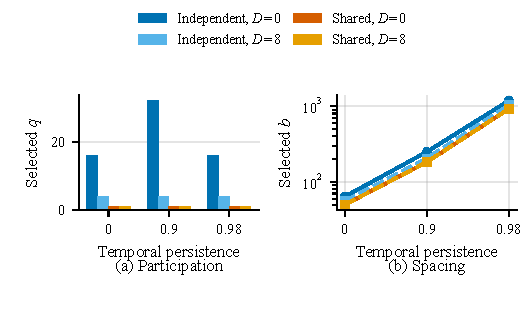
\includegraphics[width=\columnwidth]{figures/exp010b_joint_actions.pdf}
\caption{Joint actions selected by the finite-time Lyapunov certificate in EXP-010B.
The left panel reports participation and the right panel reports Markov spacing; persistence values occupy categorical positions.}
\label{fig:joint-actions}
\end{figure}

\subsection{Learning-value adaptation}
EXP-016B uses 96 finite-threshold scenario families, two model layers, eight policies, and 192 independent evaluation seeds.
All 2,752,512 rows are finite and budget-valid.
The primary estimand is the paired risk difference between probing at $B_{\rm id}$ and applying the learning-value gate in the separation phase.

Relative to information-only probing, the learning-aware controller reduces Layer-A risk by $35.24$ percent and affine delayed temporal-difference risk by $9.79$ percent.
Each reduction divides the paired risk improvement by the information-only risk.
The simultaneous one-sided lower bounds on the absolute paired improvements are $0.1612$ and $0.0577$, respectively.
Directional practical improvement occurs in 77 of 96 scenario families.
All 96 prespecified safety scenarios satisfy $S_{\rm mean}\le\epsilon_{\rm safe}$, and every trajectory obeys both resource budgets.

Fig.~\ref{fig:risk-reduction} gives reductions of $32.94$ percent with delay, $43.72$ percent when messages bind, and $30.13$ percent when transitions bind: probing is costly when it consumes the remaining learner's limiting resource.
\begin{figure}[t]
\centering
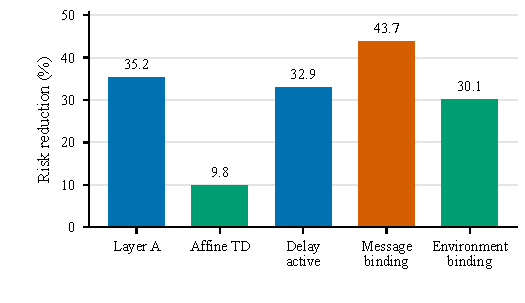
\includegraphics[width=\columnwidth]{figures/exp016b_risk_reduction.pdf}
\caption{Relative risk reductions of the learning-aware rule over information-only probing in EXP-016B.
All percentages use information-only risk as the denominator.}
\label{fig:risk-reduction}
\end{figure}

\subsection{Convergence and return-estimation curves}
TSP-CURVE-001 tests the complete joint controller on the seven-state policy-evaluation problem over a budget of 128,000 resource units.
The prespecified grid crosses persistence $\{0,0.9,0.98\}$, correlation $\{0,0.9\}$, and delay $\{0,8\}$, producing twelve cells and 41 charged-resource checkpoints per trajectory.
The fixed policies use $q\in\{1,4,16,32\}$; within every cell, each fixed $q$ receives its own certified spacing and step, so the comparison isolates the value of jointly changing participation rather than handicapping its optimizer.

Sixteen development seeds select fixed $q=4$; the locked comparison uses 64 disjoint confirmation seeds and 157,440 finite checkpoint rows.

Relative to fixed $q=4$, the joint certificate has parameter-error AUC ratio $0.9009$ with paired-bootstrap 95 percent interval $[0.8914,0.9102]$.
Its discounted-return-estimation AUC ratio is $0.8868$ with interval $[0.8678,0.9072]$.
Terminal parameter and return-estimation errors decrease by $26.48$ and $21.67$ percent, respectively.
Both AUC metrics improve in nine of twelve cells and tie in the remaining three; no cell is worse.

Fig.~\ref{fig:convergence-curves} shows the persistence-$0.9$, zero-delay slice: broad participation accelerates independent-source learning, whereas low participation avoids the shared-noise floor.
\begin{figure*}[t]
\centering
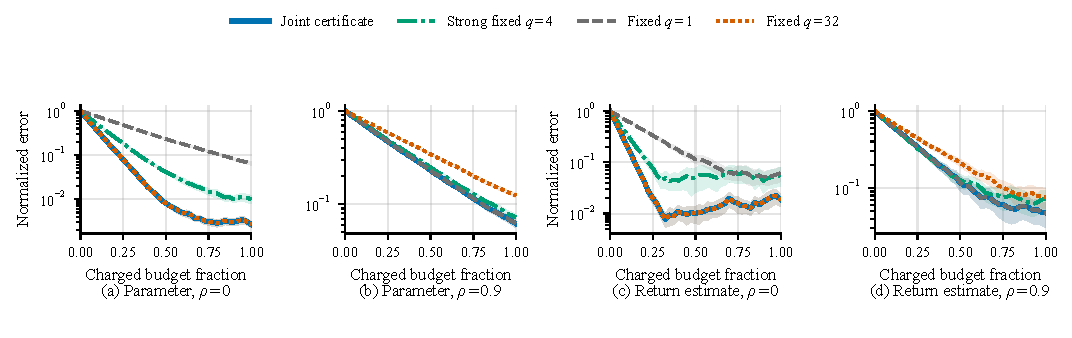
\includegraphics[width=0.96\textwidth]{figures/convergence_curves.pdf}
\caption{Held-out resource-indexed convergence in TSP-CURVE-001 for persistence $0.9$ and zero delay (64 confirmation seeds; bands are 95 percent confidence intervals).
The first two panels show parameter risk and the last two return-estimation risk, compared with the development-selected fixed $q=4$.}
\label{fig:convergence-curves}
\end{figure*}

\subsection{Transfer across cooperative policy-learning environments}
Held-out MAPPO transfer studies match message/environment budgets and charge a disjoint critic-residual probe that selects participation without evaluation return.
Both studies use eight fresh seeds per dependence regime and compare against fixed $q\in\{1,2,4,8\}$.
We compare regime-wise fixed envelopes and the strongest single fixed action for an unknown regime.

In PettingZoo \texttt{simple\_spread\_v2}, the controller commits to $q=8$ in all eight independent-stream runs and $q=1$ in all eight shared-stream runs.
It lies within $0.357$ and $0.889$ percent of the corresponding regime-wise fixed envelopes.
Against the strongest single fixed action, $q=8$, the mean of the regime--seed normalized AUC gains is $2.319$ percent; normalization precedes averaging.

In MaMuJoCo \texttt{HalfCheetah-v2/2x3}, the task-specific prespecified catalogue is $\{2,8\}$, while evaluation still includes all four fixed actions.
The controller selects $q=8$ in all eight independent-stream runs and $q=2$ in all eight shared-stream runs.
Relative to the corresponding regime-wise fixed envelopes, its AUC changes are $-0.542$ and $-0.997$ percent, both within the prespecified two-percent noninferiority margin.
When the regime is unknown, the strongest single fixed action is $q=8$.
Forming each seed's equal-regime mixture before normalization gives a mean paired AUC gain of $8.341$ percent, a one-sided 95 percent lower bound of $1.107$ percent, seven of eight positive pairs ($p=0.0352$), and a final-return gain of $4.637$ percent.

Fig.~\ref{fig:marl-return} shows the unsmoothed deterministic team-return curves against the maximum charged dual-budget fraction.
Probes consume at most $0.768$ percent of messages; selection overhead is below $10^{-6}$ of training time.
\begin{figure*}[t]
\centering
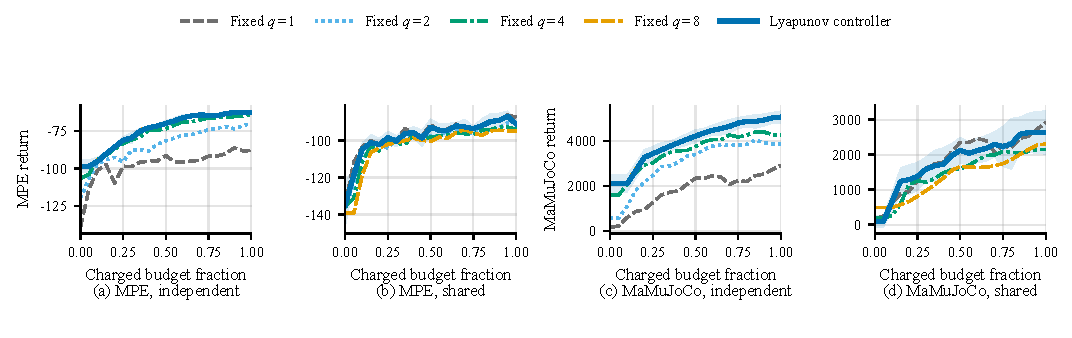
\includegraphics[width=0.96\textwidth]{figures/marl_multienvironment_returns.pdf}
\caption{Fully charged MAPPO team-return learning curves on two cooperative environments with fixed $q\in\{1,2,4,8\}$ and the Lyapunov probe-then-commit controller (eight held-out seeds per regime; shaded bands are controller 95 percent confidence intervals).
The controller selects $q=8$ for independent streams in both environments, $q=1$ for shared MPE streams, and $q=2$ for shared MaMuJoCo streams.}
\label{fig:marl-return}
\end{figure*}

\subsection{Ablations, complexity, and reproducibility}
TSP-V3-CERT-SHIELD-002 evaluates the confidence interface with 64 disjoint confirmation seeds and 157,440 checkpoint rows.
The moderate stress inflates $K_q$ and $\Omega_q$ by 10 percent and weakens the certified mixing log-rate by 0.05; the strong stress uses 25 percent and 0.10.
Both shields retain the nominal action in all twelve cells, all 24 stress-by-cell one-sided 99 percent upper means remain below the robust certificate, and neither shield changes empirical terminal risk.

The same study also isolates the finite-horizon objective.
Against one-step myopic drift, terminal parameter risk falls by 12.20 percent; against a correlation-only participation rule, it falls by 64.22 percent.
The respective ratios and paired-bootstrap 95 percent intervals are $0.878$ $[0.836,0.923]$ and $0.358$ $[0.307,0.412]$, both strictly below one.

Likelihood updates are scalar, and cached certificate search has the cost in Proposition~\ref{prop:computation}, with spectral calibration charged separately.

Controlled statistics/curves reproduce byte for byte; robustness uses eight development and 64 disjoint confirmation seeds.
Each policy-learning study has 80 finite, exactly budgeted runs spanning both regimes and all policies; all 160 runs reproduce aggregate curves byte for byte.

The ablation gains concern terminal parameter risk; the action studies separately expose correlation, spacing, and delay responses.

\section{Conclusion}
A finite-budget Lyapunov certificate jointly selects participation, physical spacing, and step size, while a learning-value gate prices dependence identification against the remaining learner.
Delayed convergence, uniform-history critic tracking, and information/learning thresholds explain the resource decisions; charged parameter-risk and cooperative-return studies demonstrate their value under correlated sampling.

\appendices
\section{Proof of the Affine Delayed Markov Bound}
\label{app:affine}
Fix a stationary action $a=(q,b,\eta)$ and condition on the history immediately before the retained joint observation.
All expectations below include the Markov observations; the delay profile is deterministic as specified in Assumption~\ref{ass:catalogue}.
Write $\bar H_k=q^{-1}\sum_iH_{i,k}$, $\bar\xi_k=q^{-1}\sum_i\xi_{i,k}$, and
\begin{equation}
v_k=e_k-\eta(\bar H_ke_k-\bar\xi_k),
\quad
r_k=\frac1q\sum_iH_{i,k}(e_{k-\tau_i}-e_k).
\label{eq:appendix-vr}
\end{equation}
Then Eq.~\eqref{eq:affine-td} is $e_{k+1}=v_k-\eta r_k$.

Total-variation duality and stationary centering give
\begin{equation}
\left\|\E[\bar\xi_k\mid\F_k]\right\|\le2G\delta.
\label{eq:conditional-bias}
\end{equation}
Moreover, stationarity and the bounded integrand imply
\begin{align}
\E[\|\bar H_ke-\bar\xi_k\|^2\mid\F_k]
&\le(2K_q+4L^2\delta)\|e\|^2\nonumber\\
&\quad+2\Omega_q+4G^2\delta.
\label{eq:second-moment-transfer}
\end{align}
Combining Eq.~\eqref{eq:conditional-bias} with the strong monotonicity of $A$ and applying Young's inequality with parameter $\mu_\delta$ yields
\begin{equation}
\E\|v_k\|^2\le a_\delta(\eta)R_k+\beta_\delta(\eta).
\label{eq:v-bound}
\end{equation}

The affine telescoping identity retains the innovation:
\begin{equation}
e_{k-\tau_i}-e_k=\eta\sum_{s=k-\tau_i}^{k-1}\left[\frac1q\sum_jH_{j,s}e_{s-\tau_j}-\bar\xi_s\right].
\end{equation}
Jensen's inequality and the almost-sure bounds in Assumption~\ref{ass:catalogue} give
\begin{equation}
\E\|r_k\|^2\le2\eta^2L^4\tau_{\rm rms}^2R_k+2\eta^2L^2G^2\tau_{\rm rms}^2.
\label{eq:r-bound}
\end{equation}
For any $\lambda>0$,
\begin{equation}
\|v_k-\eta r_k\|^2\le(1+\lambda)\|v_k\|^2+(1+\lambda^{-1})\eta^2\|r_k\|^2.
\end{equation}
Substituting Eq.~\eqref{eq:v-bound} and Eq.~\eqref{eq:r-bound} gives $\E\|e_{k+1}\|^2\le c_\lambda R_k+d_\lambda$.
The choice $\lambda=\sqrt{h_\tau/a_\delta}$ minimizes the contraction coefficient and produces Eq.~\eqref{eq:affine-cd}.
For zero delay, $r_k=0$ and the continuous limiting definitions follow directly.

Let $R_\star=d_{\rm aff}/(1-c_{\rm aff})$.
If $R_k\ge R_\star$, every new value entering the sliding envelope is at most $c_{\rm aff}R_k+d_{\rm aff}\le R_k$.
If $R_k<R_\star$, the same one-step bound keeps every new value below $R_\star$.
Thus, in both cases, each new value is at most $R_\star+c_{\rm aff}(R_k-R_\star)_+$.
After $2D+1$ updates the entire old window is replaced, giving $(R_{k+2D+1}-R_\star)_+\le c_{\rm aff}(R_k-R_\star)_+$.
Iteration gives $R_{nm}\le R_\star+c_{\rm aff}^n(R_0-R_\star)_+\le c_{\rm aff}^nR_0+R_\star$, proving Theorem~\ref{thm:affine}.

\subsection{Proof of Corollary~\ref{cor:robust-certificate}}
Write $\delta^+=C_q(r_q^+)^b$.
On the coverage event, $\delta^+\ge\delta$ and monotonicity on $\mu-2L\delta^+>0$ gives $a^+\ge a$ and $\beta^+\ge\beta$.
Evaluating the delayed Young inequality at the shared $\lambda^+=\sqrt{h/a^+}$ proves the upper recursion; separately optimized forcing terms need not be monotone.
For $\Delta\delta=\delta^+-\delta$, $\Delta K=K_q^+-K_q$, and $\Delta\Omega=\Omega_q^+-\Omega_q$,
\begin{align}
\Delta a
&=2\eta^2\Delta K+(2\eta L+4\eta^2L^2)\Delta\delta,\nonumber\\
\Delta\beta
&=2\eta^2\Delta\Omega+4\eta^2G^2\Delta\delta\nonumber\\
&\quad+4\eta G^2\left[
\frac{(\delta^+)^2}{\mu-2L\delta^+}
-\frac{\delta^2}{\mu-2L\delta}
\right],\nonumber\\
\Delta c
&=(\sqrt{a^+}+\sqrt h)^2-(\sqrt a+\sqrt h)^2.
\label{eq:certificate-perturbations}
\end{align}
For $h>0$,
\begin{align}
\Delta d
&\le(1+\sqrt{h/a^+})\Delta\beta
+\sqrt h\left(\frac1{\sqrt a}-\frac1{\sqrt{a^+}}\right)\beta\nonumber\\
&\quad+\frac{\sqrt{a^+}-\sqrt a}{\sqrt h}g,
\label{eq:certificate-delta-d}
\end{align}
and $\Delta d=\Delta\beta$ when $h=0$.
For $U(c,d)=d/(1-c)+c^n(R_0-d/(1-c))_+$, $|\partial_dU|\le(1-\bar c)^{-1}$ and $|\partial_cU|\le nR_0+\bar d(1-\bar c)^{-2}$.
The mean-value bound proves Eq.~\eqref{eq:robust-score-gap}; applying it to the upper- and exact-score minimizers gives $U_{\widehat a}\le U_{a^\star}+2\max_a\varepsilon_a$.

\subsection{Return transfer and arbitrary terminal indices}
\label{app:return}
Let $n=\lfloor N_a/(2D+1)\rfloor$.
The envelope argument keeps every later incomplete-block iterate below $\max\{R_{n(2D+1)},R_\star\}$, which is the truncated-transient form in Eq.~\eqref{eq:certificate-score}.
Since $J_\nu(w)-J_\nu(w^\star)=\psi_\nu^\top e$ for $\psi_\nu=\E_{s\sim\nu}\phi(s)$, Cauchy--Schwarz and the terminal envelope prove Corollary~\ref{cor:return}.

\subsection{Proof of Theorem~\ref{thm:tracking}}
\label{app:tracking}
Set $R_\star=d/(1-c)$ and $\Gamma_r=(Z_r-R_\star)_+$.
The explicitly assumed uniform-history drift and the positive-part replacement argument give
\begin{align}
\widetilde Z_{r+1}
&\le R_\star+c\Gamma_r,\nonumber\\
\Gamma_{r+1}
&\le(1+\chi)c\Gamma_r+\chi R_\star+(1+\chi^{-1})v^2.
\label{eq:tracking-old-target}
\end{align}
The second line follows by applying Young's inequality to the target shift and subtracting $R_\star$.
Iteration and $\Gamma_0\le Z_0$ prove Eq.~\eqref{eq:tracking-bound} whenever $\bar c=(1+\chi)c<1$.
Finally, $\widehat A_w-A^\star=\{\gamma\phi(s')-\phi(s)\}^\top(w-w_n^\star)$ and $\|\gamma\phi(s')-\phi(s)\|\le(1+\gamma)\Phi$; Cauchy--Schwarz proves Eq.~\eqref{eq:advantage-transfer}.

\subsection{Existence and complexity of the mixed controller}
\label{app:existence}
For fixed $(q,b)$, every coefficient and Eq.~\eqref{eq:certificate-score} is continuous on the declared positive-step domain.
The non-strict certification margins make that domain closed and bounded, so the extreme-value theorem applies whenever it is nonempty.
Finite enumeration across nonempty pairs gives a global minimizer.
A numerical implementation attains this oracle minimum when its scalar solver has certified global accuracy.
The $N_qN_b$ scalar searches cost $O(N_qN_bL_\eta)$ evaluations.
For rank-one $H_{i,k}$, feature inner products avoid dense matrices in update aggregation, which costs $O(qd)$ arithmetic and $O(d)$ memory.
Exact spectral moment calibration is charged separately from rank-one update aggregation.

\section{Correlation-Limited Minimax Risk}
For one round of the Gaussian location subclass, the agent average has variance $\sigma_c^2+\sigma_e^2/q$.
The $T$ round averages are independent and Gaussian with known variance, so their sample mean is minimax for squared loss over the unrestricted location family and has risk $T^{-1}(\sigma_c^2+\sigma_e^2/q)$.
Dividing the single-agent risk by this value gives Eq.~\eqref{eq:speedup}.
Since $1+(q-1)\rho\ge q\rho$ for $\rho>0$, the speedup is at most $\rho^{-1}$.

\section{Proof of the Stopped Adaptive Information Identity}
\label{app:information}
Condition on the pre-action history and realized action $A_k$.
An orthogonal rotation maps $X_k$ to $Y_k=q_k^{-1/2}\bm{1}^\top X_k$ and hypothesis-invariant standard-normal contrasts.
Because the predictable action kernels cancel, the stopped log likelihood is the sum of scalar Kalman innovation ratios, where $Y_k\sim\mathcal N(\sqrt{q_k}m^-_{j,k},V_{j,k})$.
The conditional Gaussian divergence and the bounded-stopping chain rule give Eq.~\eqref{eq:conditional-kl} and Eq.~\eqref{eq:adaptive-kl}; exchanging hypotheses gives the reverse identity.

For a decision $\widehat J$, set $p_v=\Pp_v\{\widehat J=j\}$.
Data processing gives
\begin{equation}
\KL(P_j^\pi|\F_\tau\,\|\,P_{1-j}^\pi|\F_\tau)\ge\operatorname{kl}(p_j,p_{1-j}).
\end{equation}
If both directional errors are at most $\delta$, monotonicity of binary relative entropy yields Eq.~\eqref{eq:info-constraint}.

\section{Occupation-Measure Opportunity Lower Bound}
\label{app:occupation}
Let $\Delta_j(z,a)\ge0$ be the one-step opportunity loss relative to the instance-$j$ certified oracle.
For a stopped predictable policy, define
\begin{equation}
\nu_j(G,a)=\E_j^\pi\sum_{k\le\tau}\mathbf{1}\{Z_k\in G,A_k=a\}.
\end{equation}
Every $\delta$-correct policy induces an occupation measure satisfying the controlled Kalman flow constraints,
\begin{align}
\int\mathcal{I}_{j,1-j}(z,a)\nu_j(dz,da)&\ge\operatorname{kl}(1-\delta,\delta),\nonumber\\
\int(h+q(a))\nu_j(dz,da)&\le B_{\rm msg},\nonumber\\
\int b(a)\nu_j(dz,da)+\ell\Pp_j(\tau>0)&\le B_{\rm env}.
\end{align}
Let $T_a$ be the belief transition and $\zeta_j$ the terminal belief law.
For every bounded measurable $f$, predictability and stopped telescoping give
\begin{align}
\int f(z)\zeta_j(dz)-f(z_1)
&=\int\left[\int f(z')T_a(z,dz')\right.\nonumber\\
&\left.\hspace{18mm}-f(z)\right]\nu_j(dz,da).
\label{eq:belief-flow}
\end{align}
Moreover,
\begin{equation}
\E_j^\pi\sum_{k\le\tau}\Delta_j(Z_k,A_k)
=\int\Delta_j(z,a)\nu_j(dz,da).
\end{equation}
Eq.~\eqref{eq:adaptive-kl}, Eq.~\eqref{eq:budgets}, and Eq.~\eqref{eq:belief-flow} place every admissible occupation measure in the controlled feasible set.
Taking the infimum of its exact loss over that larger set proves Proposition~\ref{prop:occupation}.

\section{Proof of the Main Learning-Value Guarantee}
\label{app:main}
Let $\mathcal H_d$ be the complete probe history.
The declared conditional certificate gives $\E_j[\|e_{\rm LA}\|^2\mid\mathcal H_d]\le\overline R_j(\widetilde a_{\widehat J};B_d^D,D)$ for either selected action.
The right side is at most $\overline R_j^{\rm sel}+\mathbf1\{\widehat J\ne j\}W_j(d)$.
Taking expectation and using the directional error bound proves Eq.~\eqref{eq:main-risk}.

Subtracting the full-budget all-agent certificate and using Eq.~\eqref{eq:value-decomposition} gives
\begin{equation}
\E_1\|e_{\rm LA}\|^2-\overline R_1^{\rm all}(B,D)
\le C_1^{\rm probe}+C_1^D-G_1+\delta W_1<0.
\end{equation}
The same decomposition on instance zero is bounded above by $\epsilon_{\rm safe}(d)\le\bar\epsilon$.
The fallback statement follows directly from the strict admission rule.

\section{Proof of the Threshold Sandwich}
\label{app:threshold}
For the independently initialized Gaussian running mean, let $c_a=\max\{(h+q)/\beta_m,b/\beta_e\}$ and $r=\lambda^b$.
The exact horizon is $N_a=s/c_a+O(1)$, with bounded terminal charges and rounding.
Eq.~\eqref{eq:mean-risk} and Eq.~\eqref{eq:geometric-correlation-sum} give $K_j(a)=c_a\{q^{-1}+\theta_j(1+r)/(1-r)\}$ and a uniform $O(s^{-2})$ remainder.
Removing probe charge $v$ changes $N_a$ by $O(v+1)$ and hence risk by $O((v+1)/s^2)$ for $s\ge s_0(v+1)$; compact persistence and the finite catalogue make these constants uniform.
Thus the phase-theorem risk conditions have a concrete Gaussian realization, separately from the constant-step affine certificate.
Write $d_\delta=\operatorname{kl}(1-\delta,\delta)$.
Write $r_0=1-\gamma<1$ and $Q=\max{\cal Q}$.
Under either true instance, the predictable spacing gives $\|C_{S_k}\|_{L^2}\le r_0\|C_{S_{k-1}}\|_{L^2}+\sqrt{\theta_+}$, hence a uniform bound $M_C=\sqrt{\theta_+}/(1-r_0)$.
The normalized observation $Y_k/\sqrt{q_k}$ has $L^2$ norm at most $M_C+1$.
For either candidate filter, write its posterior mean as $(1-t_{j,k})m^-_{j,k}+t_{j,k}Y_k/\sqrt{q_k}$, with predictable $0\le t_{j,k}\le1$.
Prediction multiplies this mean by a factor of magnitude at most $r_0$; the triangle inequality therefore bounds both predictive means uniformly in $L^2$ by $M_F=r_0(M_C+1)/(1-r_0)$, starting from zero.
Both predictive variances are at most $\theta_+$, so $1\le V_{j,k}\le V_+=1+Q\theta_+$.
Eq.~\eqref{eq:conditional-kl} now gives the expected, rather than pointwise, bound $\E_j\mathcal I_{j,1-j}(Z_k,A_k)\le i_+$, where $i_+=(\log V_++V_++4QM_F^2)/2$ is finite.
Extend a stopped rule predictably after stopping; nonnegativity and its deterministic budget bound $n_{\max}(s)\le c_Bs$ imply $\E_j\sum_{k\le\tau}\mathcal I_{j,1-j}\le i_+n_{\max}(s)$.
Together with Eq.~\eqref{eq:info-constraint}, this expected-information bound proves $B_N\ge c_Nd_\delta$ over Gaussian observation histories.
The fixed probe has information at least $i_->0$, so $n_\delta=\lceil i_-^{-1}\log(1/\delta)\rceil$ observations suffice and cost at most $c_pn_\delta+D_{\max}$.
Continuity of $\log(1/\delta)/d_\delta$ gives $n_\delta\le c_0+c_1d_\delta\le c_0+c_2B_N$.
Write $u_\delta\le c_pn_\delta+D_{\max}$ for the full probe charge.
The assumed expansion and budget-shift inequality give a high-instance improvement over the full-budget fallback certificate of at least $g_{\min}/s-\{2M+L(u_\delta+1)\}/s^2-\delta w_+/s$.
It is strictly positive for $s>\{4M+2L(u_\delta+1)\}/g_{\min}$, also requiring $s\ge s_0(u_\delta+1)$.
On instance zero, the assumed coefficient ordering gives $\epsilon_{\rm safe}\le\{2M+L(u_\delta+1)\}/s^2+\delta_0w_+/s$.
Thus $s\ge\sqrt{2\{2M+L(u_\delta+1)\}/\bar\epsilon}+2\delta_0w_+/\bar\epsilon$ suffices.
Using $2\sqrt{xy}\le x+y$, all three requirements are bounded by a class-constant multiple of $n_\delta+B_{\rm oracle}+B_\epsilon+1$.
Taking the maximum proves the upper bound in Eq.~\eqref{eq:threshold-sandwich}; its lower bound follows because every admitted $\delta$-correct probe obeys both information constraints.


\bibliographystyle{IEEEtran}
\bibliography{references}
\end{document}
